\documentclass{article}
\usepackage[utf8]{inputenc}
\usepackage[T1]{fontenc}
\usepackage[russian]{babel}
\usepackage{tikz}
\usepackage{graphicx}
\usepackage{titlesec}
\usepackage{amsfonts}
\usepackage{amsmath}
\usepackage[left=2cm,right=2cm,
    top=2cm,bottom=2cm,bindingoffset=0cm]{geometry}
\renewcommand{\thesection}{\arabic{section}}
\titleformat{\section}{\large\bfseries}{\thesection}{1em}{}
\title{Интегрирование}
\author{Каренин Константин Витальевич}
\date{22.05.2024}
\begin{document}

\begin{titlepage}
    \centering
    \vspace*{0.5 cm}
    
    \textsc{\LARGE \textbf{Математический анализ}}
    \vspace{1.5cm}
    
    \rule{\linewidth}{0.2 mm} \\[0.4 cm]
    { \huge \bfseries Функции нескольких переменных}
    \rule{\linewidth}{0.2 mm} \\[1.5 cm]
    
    \Large Выполнили: \\
    Каренин Константин \\
    Темиров Тимур \\
    Гонин Сергей \\
    Малышева Алиса \\
    
    \vspace{0.5cm}
    
    Группа: М3104
    
    \vspace{0.5cm}
    
    Преподаватель: Сарычев Павел
    
    \vspace{0.5cm}
    
    Университет ИТМО
    
    \vfill

    
\includegraphics[height=70px]{logo.jpg}
    
    22.05.2024
    
\end{titlepage}

\setcounter{page}{2}

% task 1
\newpage
    \section{Изобразите в графическом калькуляторе поверхность, заданную уравнением $z = \ln(x^2 + 4 y^2)$}
    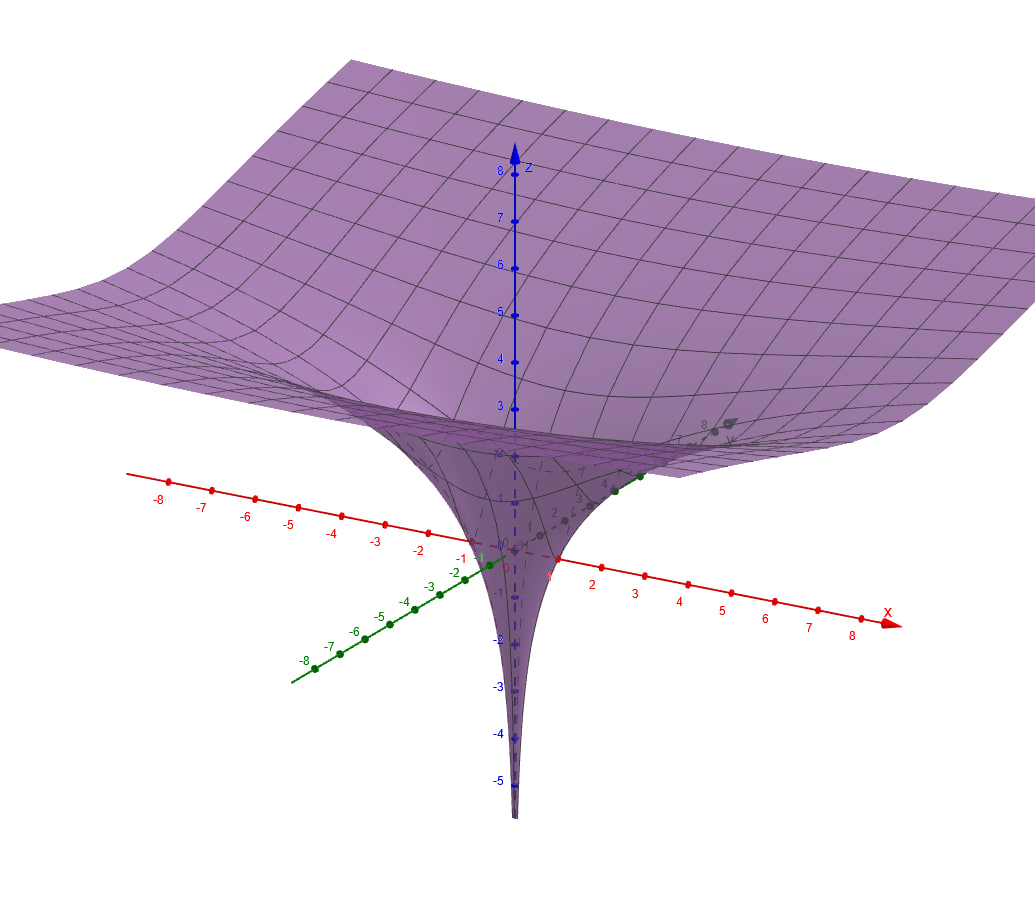
\includegraphics[height=200px]{ргр_матан2_11.jpg}
    
    \subsection{Найдите область определения функции $f (x, y)$}
    Функция определена тогда и только тогда, когда $x^2 + 4y^2 > 0$\\
    Сумма квадратов положительна, если хотя бы один из них не равен 0. Т.к. $a^2 \geq 0$, для любых $a \in \mathbb{R}$, то нам нужно исключить из области определения единственный случай: 
    \begin{equation*}
        \begin{cases}
            x^2 = 0 \\
            4y^2 = 0
        \end{cases}
        \Rightarrow
        \begin{cases}
            x = 0 \\
            y = 0 \\
        \end{cases}
    \end{equation*}
    Таким образом $x^2 + 4y^2 >0 \forall (x, y) \in \mathbb{R}^2 : (x, y) \neq (0, 0)$\\
    $D(f(x, y)) = \{(x, y) \in \mathbb{R}^2 : (x, y) \neq (0, 0) \}$
    
    \subsection{Изобразите на одном листе семейство линий уровня $f (x, y) = c$ функции $f (x, y)$. Для построения выберите 3 –
    4 значения $c$. Определите тип построенных кривых. Если различным c соответствуют кривые разных типов,
    изобразите все типы линий уровня.}
    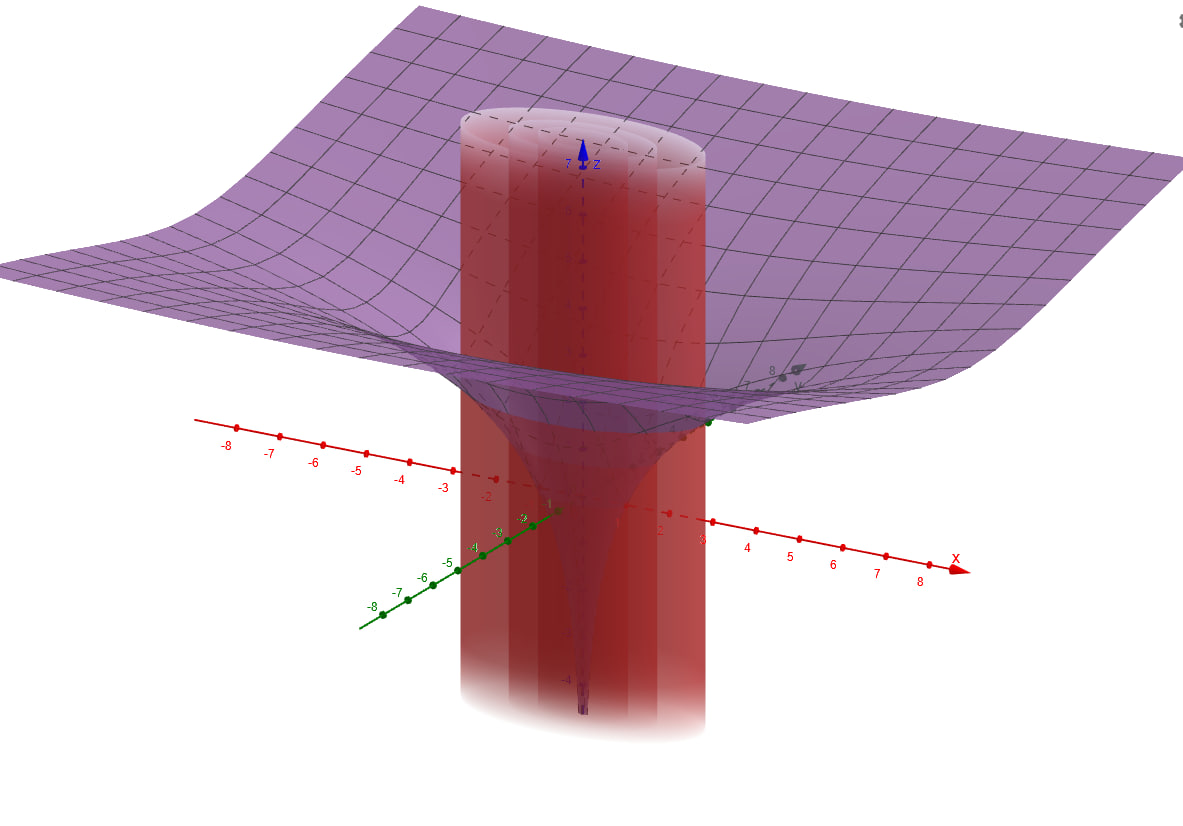
\includegraphics[height=200px]{ргр_матан2_12.jpg} \\ \\
    Линия уровня $f(x, y)$ определяется уровнем $f(x, y) = c; \; \ln(x^2 +4y^2) = c; \; x^2 + 4y^2 = e^c$ \\
    Для различных значений $c$ получаем семейство эллипсов $x^2 +4y^2 = k$, где $k = e^c = const$\\
    Выберем несколько значений $c$ и запишем для них уравнения эллипсов при:\\
    $c=0: x^2 +4y^2 = 1$\\
    $c=1: x^2 +4y^2 = e$\\
    $c=2: x^2 +4y^2 = e^2$   
    
    \subsection{Выберите на поверхности какую-либо точку $M_0(x_0, y_0, z_0)$, не являющейся ни особой, ни стационарной, и дока-
    жите это по определению.}
    Точка $M_0(x_0, y_0, z_0)$ не является ни особой, ни стационарной. Рассмотрим точку $M_0$ для которой $x_0 = 1, y_0 = 0$, тогда $z_0 = f(1, 0) = \ln (1^2 + 4 \cdot 0^2) = \ln 1 = 0$. Докажем по определению, что она не особая и не стационарная.\\
    Особая точка ФНП - это точка в которой функция либо не определена, либо не имеет всех частных производных. К таким точка относятся: те в которых функция не определена и те в которых функция разрывна (их предел не существует либо бесконечен), а также те в которых функция не имеет частных производных, либо частные производные не определены или не непрерывны.\\
    $M_0 (1, 0, 0) \in D(f(x, y))$ - функция в данной точке определена\\
    Найдём частные производные:\\
    $f_x'=\frac{2x}{x^2 + 4y^2}$\\
    $f_y'=\frac{8y}{x^2 + 4y^2}$\\
    В точке $(1, 0, 0):$\\
    $f_x'(1, 0, 0)=\frac{2 \cdot 1}{1^2 + 4 \cdot 0^2}$\\
    $f_y'(1, 0, 0)=\frac{8 \cdot 0}{1^2 + 4 \cdot 0^2}$\\
    Частные производные существуют \Rightarrow $M_0$ - не особая точка.

    Стационарная точка ФНП - это точка в которой все первые частные производные равны 0. Тоесть в этой точке градиент равен 0. Для нашей $M_0$ частная производная по $x \; f_x' \neq 0$, градиент $\nabla f(1, 0)=(2, 0) \neq 0 \Rightarrow M_0$ - не стационарная точка
    
    \subsection{Найдите вектор $\overrightarrow{m} \in \mathbb{R}^2$, показывающий направление наискорейшего подъёма (спуска) в точке $M_0$.}
    Направление наискорейшего подъема совпадает с направлением градиента функции $f: \nabla f(1, 0) = (2, 0) \Rightarrow \overrightarrow{m} = (2, 0)$
    
    \subsection{Изобразите линию уровня $f (x, y) = z_0$ и направление $\overrightarrow{m}$ . Проверьте их ортогональность.}
    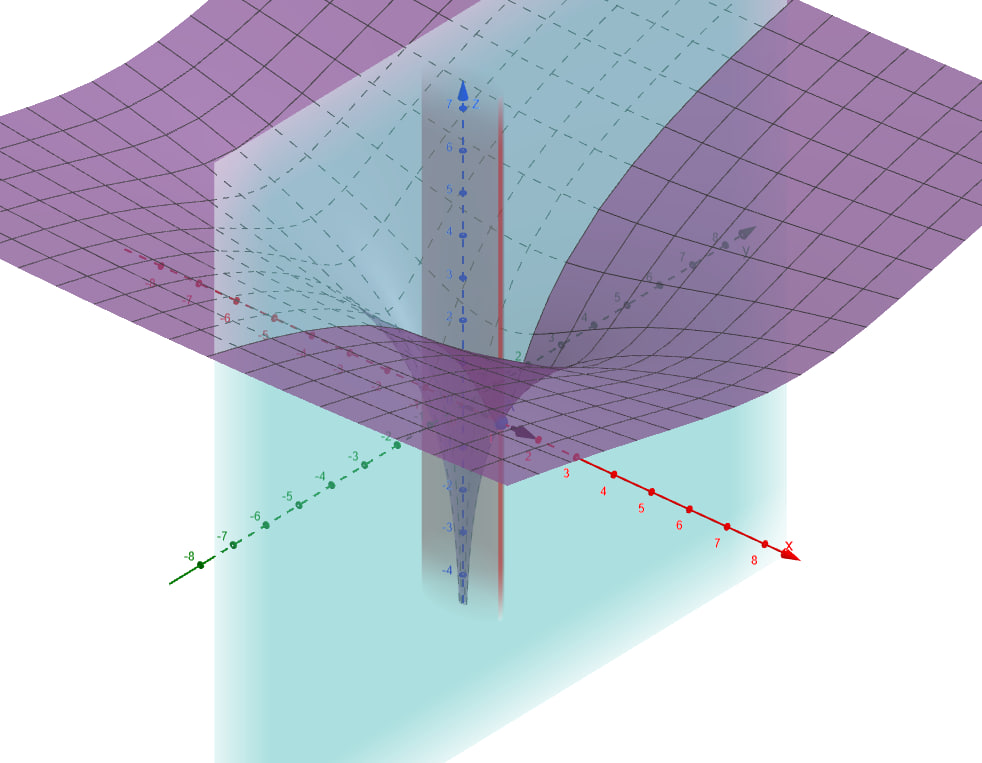
\includegraphics[height=200px]{ргр_матан2_13.jpg} \\
    Линия уровня, проходящая через $M_0$ задается уравнением: $x^2 + 4y^2 = 1$ и имеет касательную плоскость $x = 1$ в точке $M_0$ параллельную оси $Oy$\\
    Вектор $\overrightarrow{m} = (2, 0)$ - параллелен оси $Ox:$ проверим что $\overrightarrow{m}$ и направляющий вектор касательной в точке $M_0$ ортогональны\\
    Произведение $(0, 1) \cdot (2, 0) = 2 \cdot 0 + 0 \cdot 1 = 0$ действительно, вектор направления подъема и линия уровня в точке $M_0$ ортогональны
    

    
% task 2
\newpage
    \section{Дано векторное поле $\overrightarrow{H} = (y \cos(xy), x \cos (xy))$}
    \subsection{Убедитесь, что данное векторное поле потенциально.}
    Чтобы показать, что поле потенциально нужно убедиться, что $rot \overrightarrow{H}=0$
    \begin{equation*}
        rot \overrightarrow{H} =
        \begin{vmatrix}
            \overrightarrow{i} & \overrightarrow{j} & \overrightarrow{k}\\
            \frac{\partial}{\partial x} & \frac{\partial}{\partial y} & \frac{\partial}{\partial Z}\\
            y\cos(xy) & x\cos(xy) & 0\\
        \end{vmatrix}
        = \overrightarrow{j} \frac{\partial}{\partial z} y \cos(xy) + \overrightarrow{k} \frac{\partial}{\partial x} x \cos (xy) - \overrightarrow{k} \frac{\partial}{\partial y} y \cos (xy) - 0 - 0 =
    \end{equation*}
    \begin{equation*}
        = \overrightarrow{k} (\cos(xy) - xy \sin(xy) - \cos(xy) + xy \cos(xy)) = 0 \Rightarrow \overrightarrow{H} \text{ - потенциально}
    \end{equation*}
    
    \subsection{Найдите уравнения векторных линий. Изобразите векторные линии на рисунке.}
    Пусть $l: \overrightarrow{r} = \overrightarrow{r} (M) \forall M \in \mathbb{R}^3$, где $M(x_0, y_0, z_0)$ \\
    $l$ - векторная линия, если $d\overrightarrow{r}(dx, dy) \text{||} \overrightarrow{H}$\\
    То есть $\frac{dx}{y\cos(xy)} = \frac{dy}{x\cos(xy)}$\\
    \begin{equation*}
        \begin{cases}
            z = C_1\\
            x \cos(xy) dx = y \cos(xy) dy\\            
        \end{cases}
    \end{equation*}
    \begin{equation*}
        \int (x \cos (xy))dx = 
        \left[
        \begin{array}{cc}
            u = x & u = \frac{1}{y}\sin(xy) \\
            du = \cos(xy) dx & du = dx \\ 
        \end{array}
        \right] = 
        \frac{x}{y} \sin (xy) + \frac{1}{y^2} \cos (xy) + C
    \end{equation*}
    \begin{equation*}
        \int (y \cos (xy)) dy = \frac{y}{x} \sin (xy) + \frac{1}{x^2} \cos(xy) + C
    \end{equation*}
    \begin{equation*}
        \begin{cases}
            z = C_1\\
            \frac{x}{y} \sin(xy) + \frac{1}{y^2} \cos(xy) = \frac{y}{x} \sin (xy) + \frac{1}{x^2} \cos (x^2) + C_2
        \end{cases}
    \end{equation*}
    \begin{equation*}
        \begin{cases}
            z = C_1\\
            (\frac{x}{y} - \frac{y}{x}) \sin (xy) + (\frac{1}{y^2} - \frac{1}{x^2}) \cos (xy) = C_2
        \end{cases}
    \end{equation*}
    \begin{equation*}
        \begin{cases}
            z = C_1\\
            (x^2 - y^2)(\frac{1}{xy}\sin (xy) + \frac{1}{x^2y^2}\cos(xy)) = C_2
        \end{cases}
    \end{equation*}
    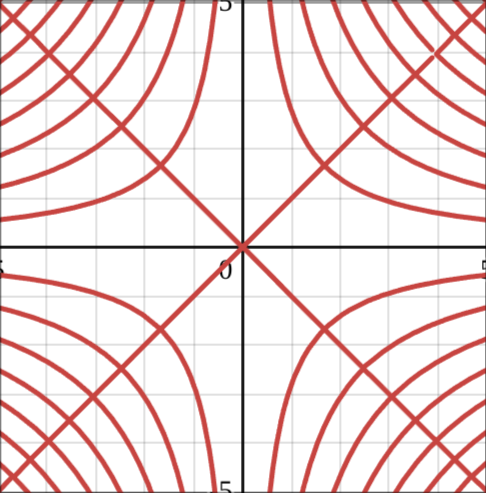
\includegraphics[height=150px]{ргр_матан2_21.png}
    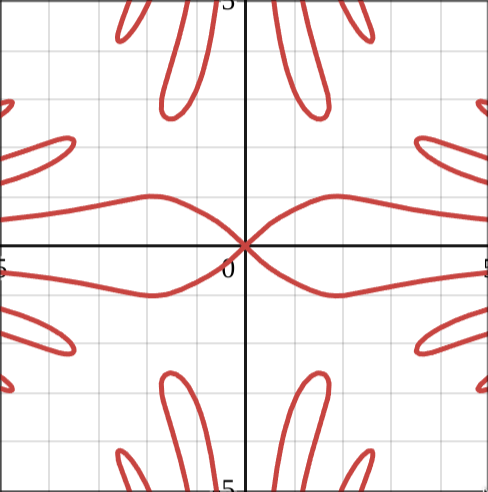
\includegraphics[height=150px]{ргр_матан2_22.png}
    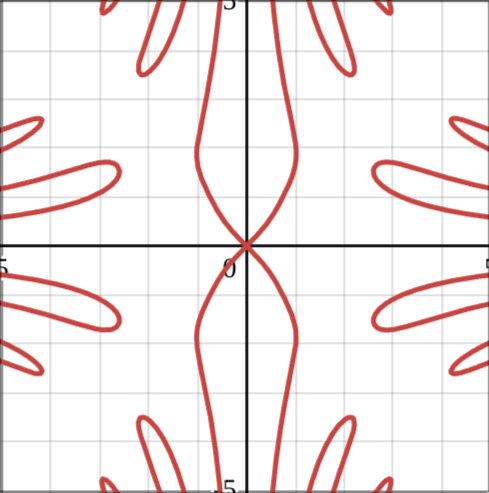
\includegraphics[height=150px]{ргр_матан2_23.png}
    
    \subsection{Найдите потенциал поля при помощи криволинейного интеграла.}
    $\exists u$, такое $u(x,y,z)$ - потенциал $\overrightarrow{F}$, если \\
    \overrightarrow{F} = \overrightarrow{grad} u = \frac{\partial u}{\partial x}\overrightarrow{} + \frac{\partial u}{\partial y}\overrightarrow{j} + \frac{\partial u}{\partial z} \overrightarrow{k}
    
    \begin{equation*}
        \begin{cases}
            \frac{\partial u}{\partial x} = y cos(xy) \\
            \frac{\partial u}{\partial y} = x cos(xy) \\
            \frac{\partial u}{\partial z} = 0\\
        \end{cases}
        \text{интегрируем}
        \begin{cases}
            u_x = \int_{x_0}^x y cos(xy) dx \\
            u_y = \int_{y_0}^y  x cos(xy) dy \\
            u_z = 0\\
        \end{cases}
    \end{equation*}
    \begin{equation*}
        \begin{cases}
            u_x = \frac{x}{y} sin(xy) + \frac{1}{yz} cos(xy) \bigg|_{x_0}^x \\
            u_y = \frac{x}{y} sin(xy) + \frac{1}{xz} cos(xy) \bigg|_{y_0}^y \\
            u_z = 0
        \end{cases}
    \end{equation*}
    Пусть M = $(2\sqrt{\pi}, 2\sqrt{\pi})$
    \begin{equation*}
        \begin{cases}
            u_x = \frac{x}{y} sin(xy) + \frac{1}{yz} cos(xy) - \frac{1}{4\pi} \\
            u_y = \frac{x}{y} sin(xy) + \frac{1}{xz} cos(xy) - \frac{1}{4\pi} \\
            u_z = 0
        \end{cases}
    \end{equation*}
    Тогда $u(x,y) = \frac{x}{y} sin(xy) + \frac{1}{yz} cos(xy) + \frac{y}{x} sin(xy) + \frac{1}{xz} cos(xy) + C$ \\
    \subsection{Найдите уравнения линий уровня потенциала(эквипотенциальных линий). Изобразите линии уровня потенциала.}
    Пусть $z = u(x,y), \forall \, C = 0$\\
    $
    z = 0 
    \;\;\;\;\;\;\;\;\;\;\;\;\;\;\;\;\;\;\;\;\;\;\;\;\;\;\;\;\;\;\;\;\;\;\;\;
    \;\;\;\;\;\;\;\;\;\;\;\;\;\;
    z = 1
    \;\;\;\;\;\;\;\;\;\;\;\;\;\;\;\;\;\;\;\;\;\;\;\;\;\;\;\;\;\;\;\;\;\;\;\;
    \;\;\;\;\;\;\;\;\;\;\;\;\;\;
    z = -1$ \\
    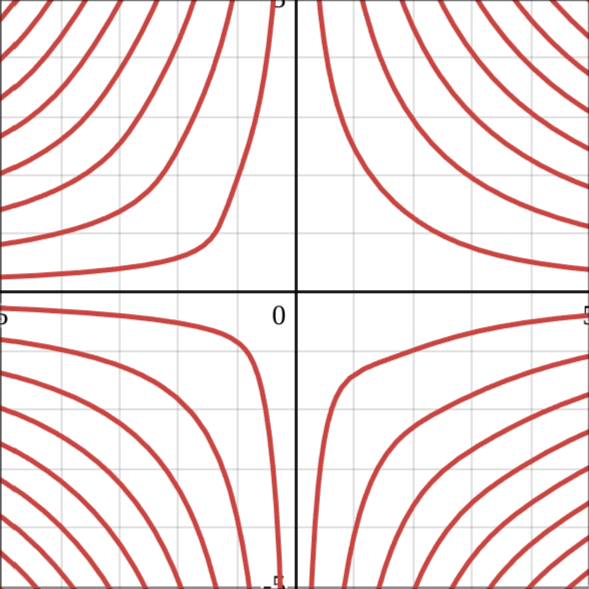
\includegraphics[height=150px]{ргр_матан2_24.png} 
    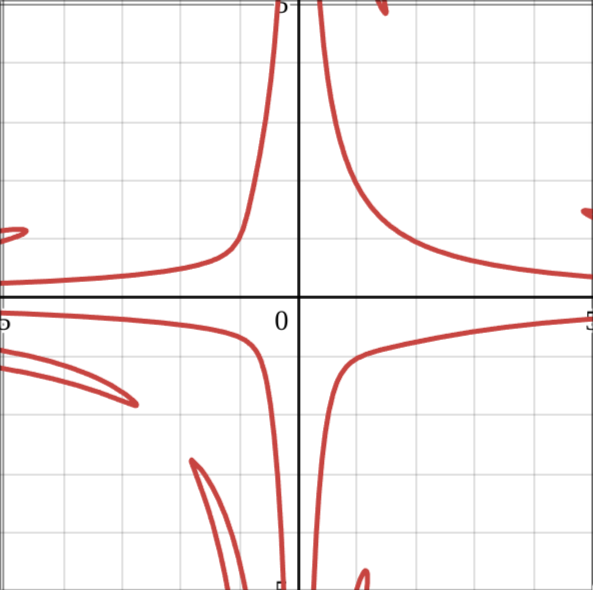
\includegraphics[height=150px]{ргр_матан2_25.png} 
    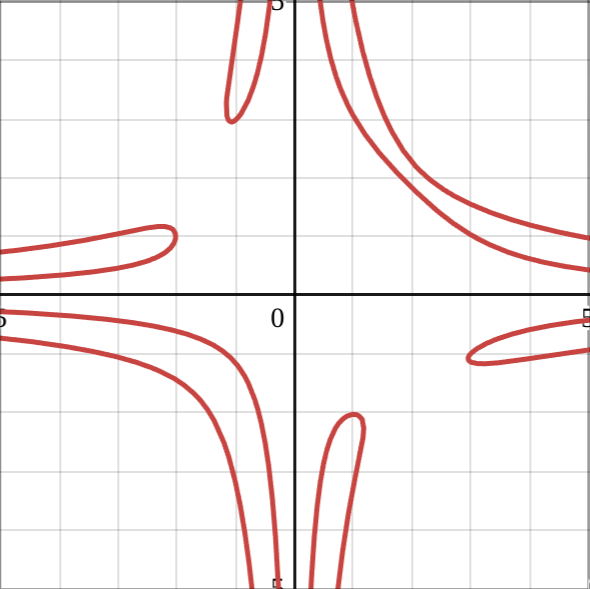
\includegraphics[height=150px]{ргр_матан2_26.png} 
    \subsection{Докажите ортогональность найденных векторных линий поля и линий уровня потенциала. Проиллюстрируйте ортогональность на графике.}
    Из уравнения линий уровней: 
    \begin{equation*}
        u(x,y) = C \\
        du = 0 \\
    \end{equation*}
    \begin{equation*}
        du = \frac{\partial u}{\partial x} dx + \frac{\partial u}{\partial y} dy = \overrightarrow{grad} u \cdot d\overrightarrow{r} = 0
    \end{equation*}
    \begin{equation*}
        \begin{cases}
            \overrightarrow{grad} u \perp d \overrightarrow{r} \\
            \overrightarrow{grad} = \overrightarrow{H} \\
        \end{cases}
        \Rightarrow
        \overrightarrow{H} \perp d\overrightarrow{r}
    \end{equation*}
    Так как касательный вектор к $u(x,y) =C $ перпендикулярно вектору поля, то векторные линии ортогональны линиям уравнения потенциала.\\
    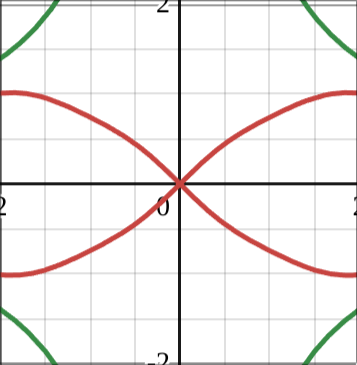
\includegraphics[height=200px]{ргр_матан2_27.jpg} \\
    Если наклонить голову и присмотреться, то можно будет заметить ортогональность
    \subsection{Выберите какую-либо векторную линию поля и зафиксируйте на ней точки $A$ и $B$, выбрав для них числовые
    координаты. Вычислите работу поля вдоль этой линии, используя найденный в пункте 3 потенциал.}
    Пусть $A(\sqrt{\pi}, \sqrt{\pi})$ $B(\sqrt{2\pi}, \sqrt{2\pi})$ \\
    $W = u(B) - u(A) = \frac{1}{\pi} + \frac{2}{\pi} = \frac{3}{\pi}$ Дж

% task 3
\newpage
    \section{Дано тело $T: y + \sqrt{1 - x^2 - z^2} = 0$, ограниченное некоторыми поверхностями $y + 2\sqrt{x^2 + z^2} = 2; \; \overrightarrow{a} = \cos(zy) \overrightarrow{i} + x \overrightarrow{j} + (e^y^2 - 5z)\overrightarrow{k}; \; \alpha = ABC; \; l=Oy$.}
     \begin{equation*}
     T:
        \begin{cases}
            y + \sqrt{1-x^2-z^2} = 0 \\
            y + 2 \cdot \sqrt{x^2 + z^2} = 0
        \end{cases}
    \end{equation*}
    \subsection{Изобразите тело T на графике в пространстве.}
    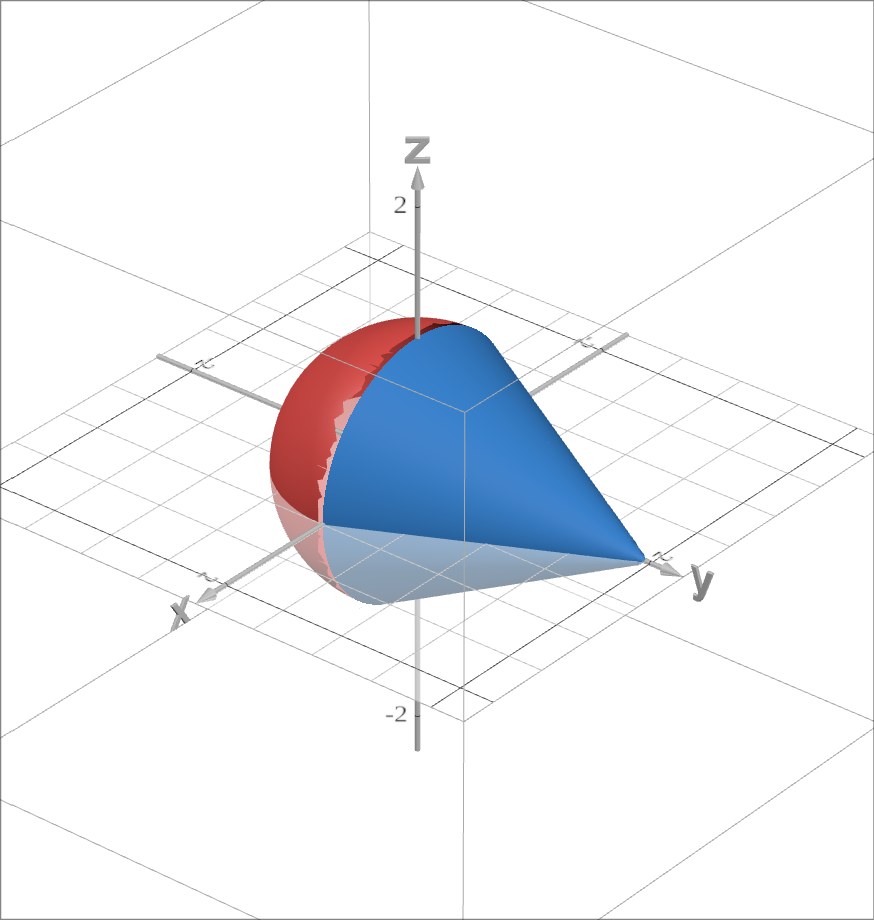
\includegraphics[height=200px]{ргр_матан2_31.jpg} \\

    \subsection{Вычислите поток поля $\overrightarrow{a}$ через боковую поверхность тела $T$, образованную вращением дуги $\alpha$ вокруг оси $l$ в
    направлении внешней нормали поверхности тела $T$.}
    $\overrightarrow{a} = \cos(zy)\overrightarrow{i} + x\overrightarrow{j} + (e y^2 - 5z)\overrightarrow{k}$ \\
    $\alpha = ABC$ \\
    $l = Oy;$ \\
    Посчитаем поток: \\
    $\Phi =  \int\int_{S}{(\overrightarrow{a}, d\overrightarrow{\sigma})}$\\
    Спроектируем $\sigma$ на $xoz$\\
    $\int\int_{S}(\overrightarrow{a}, d \overrightarrow{S_i}) = \int\int_{S}(\overrightarrow{a},\overrightarrow{h}) ds$\\
    Нормаль сферы на бесконечно малом участке лежит на одной прямой с радиус-ветором от $\Phi$ до данного кусочка, соответственно, нормаль считается так: \\
    $\overrightarrow{n} = x\overrightarrow{i} + y\overrightarrow{j} + z\overrightarrow{k}$ (поскольку сфера единичная) \\
    Воспользуемся теоремой Гаусса-Остроградского: \\
    $ \int\int_{S}(\overrightarrow{a}, d) = \int\int_V\int div\overrightarrow{a}dV$ \\
    $div\overrightarrow{a} = \frac{\partial a}{\partial x} + \frac{\partial a}{\partial y} + \frac{\partial a}{\partial z}
    = \frac{\partial \cos(yz}{\partial x} + \frac{\partial x}{\partial y} + \frac{\partial a(ey^2 - 5z)}{\partial z} = -5$ \\
    $-5\int\int_{V}\int dV = -10\pi$ 
    



    
% evaluation paper
\newpage
\[
\renewcommand{\arraystretch}{2}
\begin{tabular}{| c | c |}
 \hline
    \hugeУчастник & \hugeВклад в \% \\
 \hline
    \hugeКаренин Константин & \huge25 \\
 \hline
    \hugeГонин Сергей & \huge25 \\
 \hline
    \hugeТемиров Тимур & \huge25 \\
 \hline
    \hugeМалышева Алиса & \huge25 \\
 \hline
\end{tabular}
\]
\end{document}